\section{Respiratory Sinus Arrhythmia from RR-Intervals}
\subsection{PSD of RRI data}
After processing the ECG data to RRI data in three trails, the standard and the Bartlett averange periodograms are plotted with rectangular window length $L \in$ [$50s$, $100s$, $150s$]. Based on the analysis in section 1.2.2, the standard periodogram has relatively large variance and less leakage. With the decreasing length of window, the periodogram is tending to be smooth, resulting in both low variance and precision.
\begin{figure}[htb]
     \centering
     \begin{subfigure}{0.4\textwidth}
         \centering
         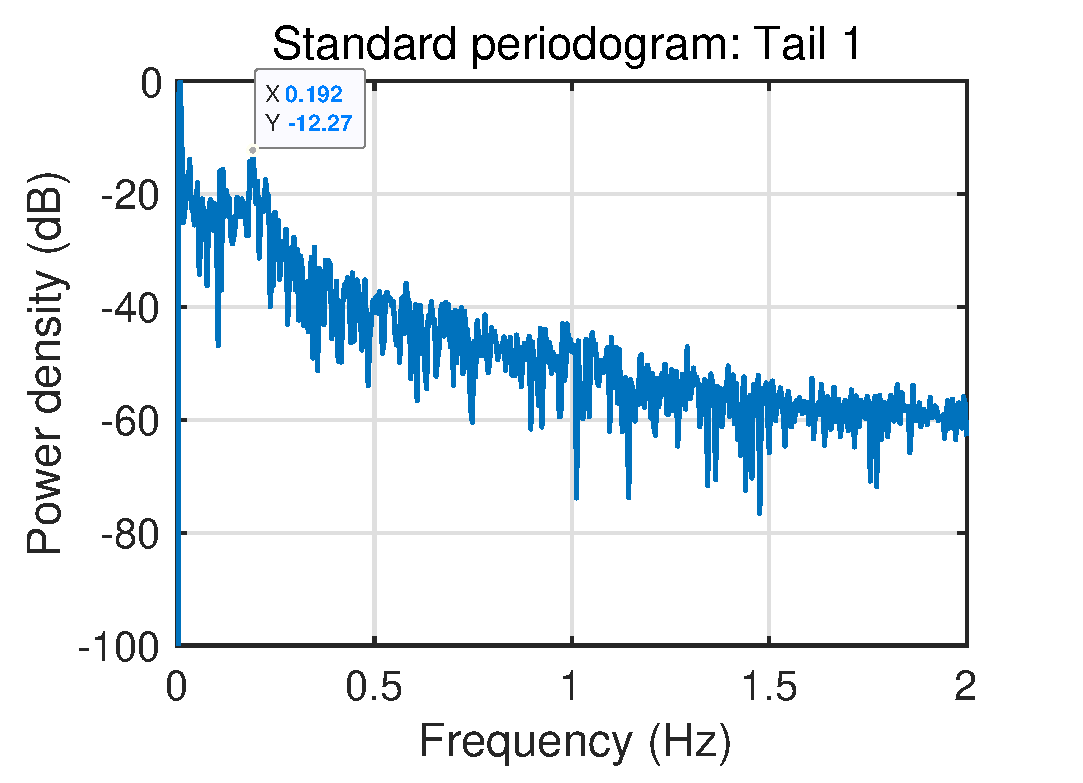
\includegraphics[width=\textwidth]{fig/15/15a1.eps}
     \end{subfigure}
     ~
     \begin{subfigure}{0.4\textwidth}
         \centering
         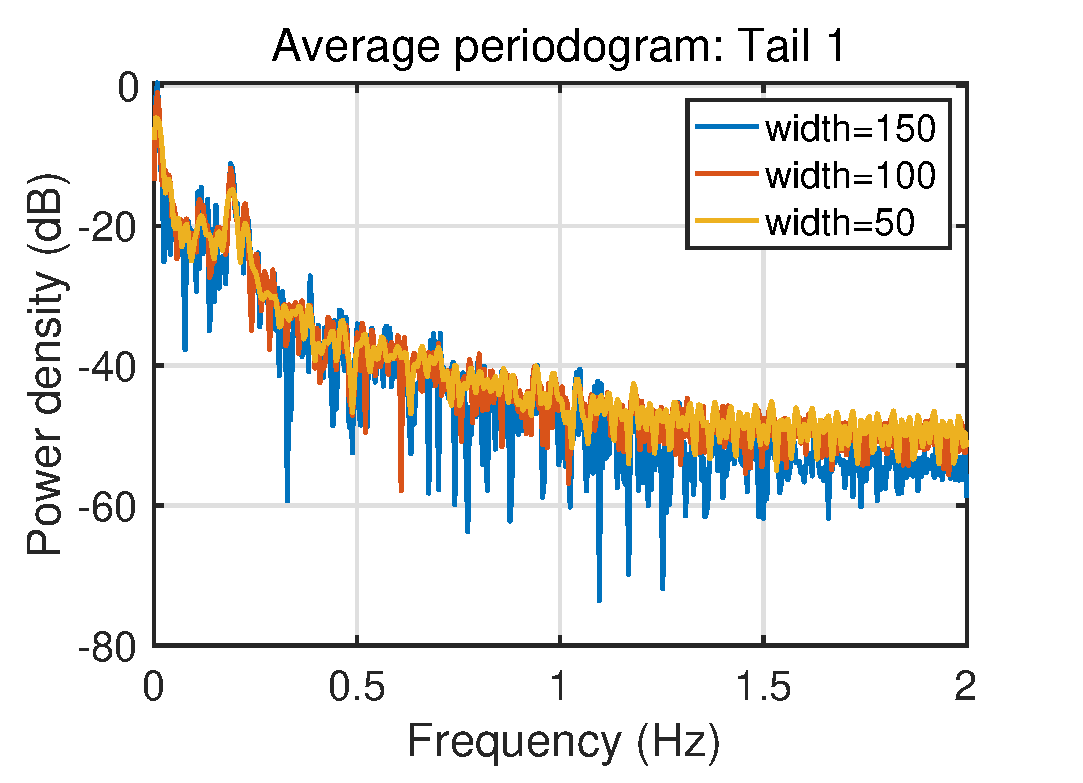
\includegraphics[width=\textwidth]{fig/15/15a2.eps}
     \end{subfigure}
     ~
     \begin{subfigure}{0.4\textwidth}
         \centering
         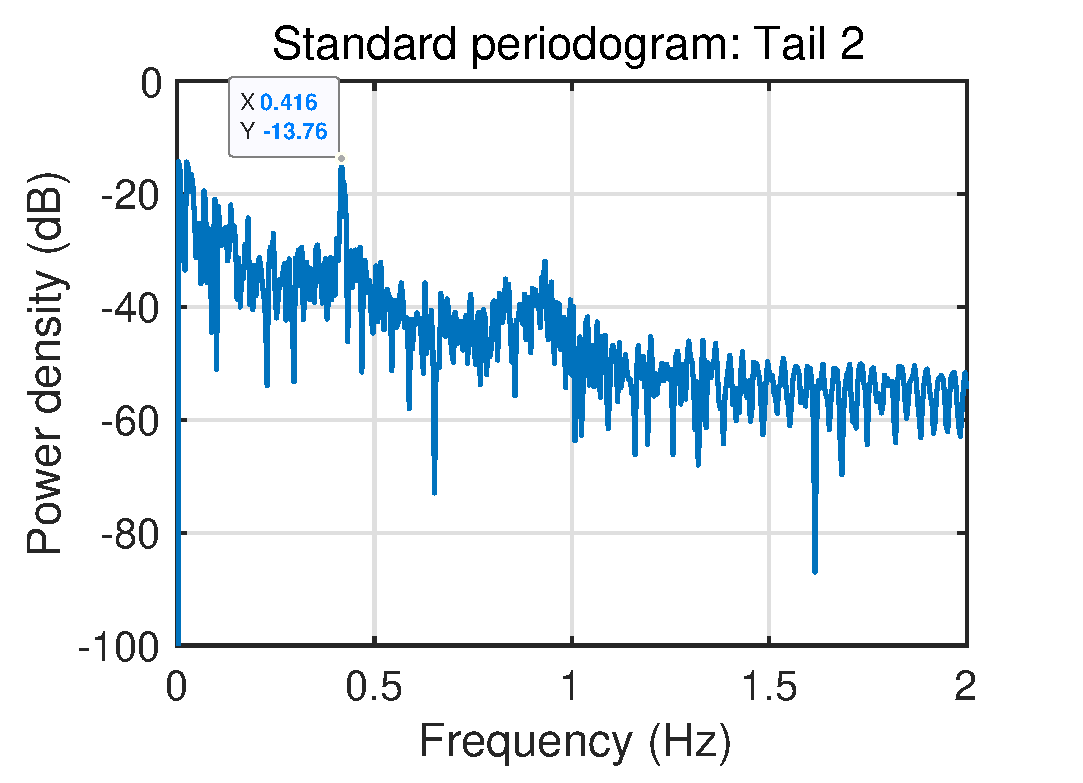
\includegraphics[width=\textwidth]{fig/15/15a3.eps}
     \end{subfigure}
     ~
     \begin{subfigure}{0.4\textwidth}
         \centering
         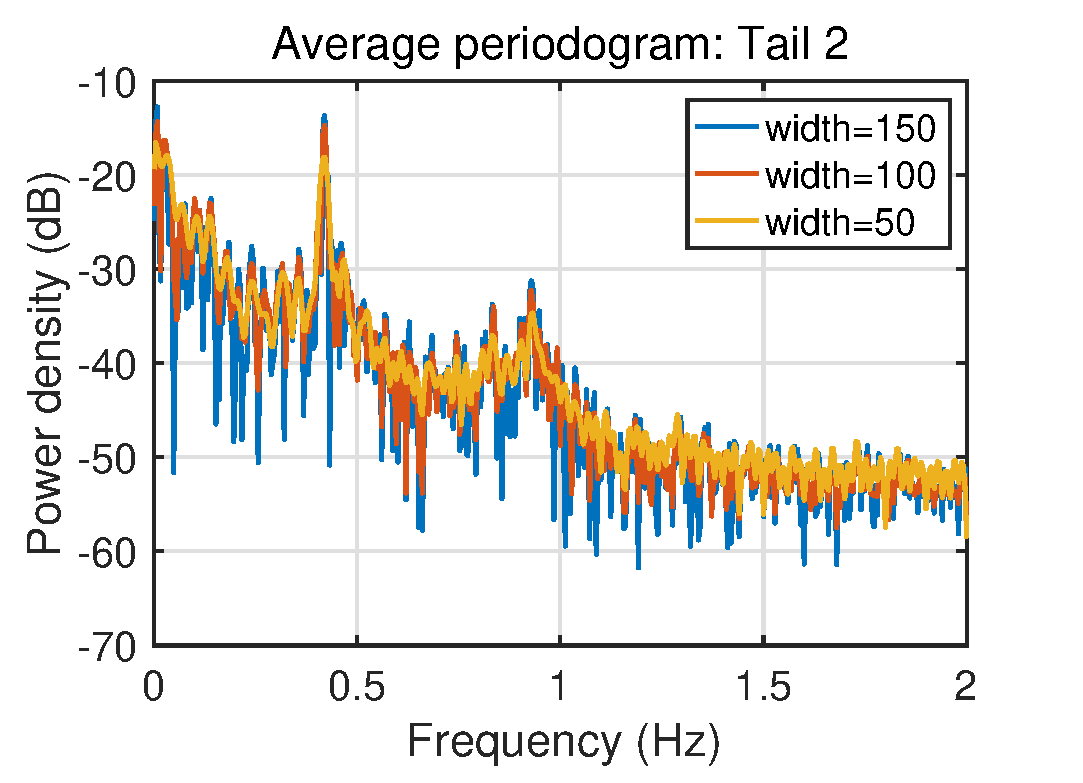
\includegraphics[width=\textwidth]{fig/15/15a4.eps}
     \end{subfigure}
     ~
     \begin{subfigure}{0.4\textwidth}
         \centering
         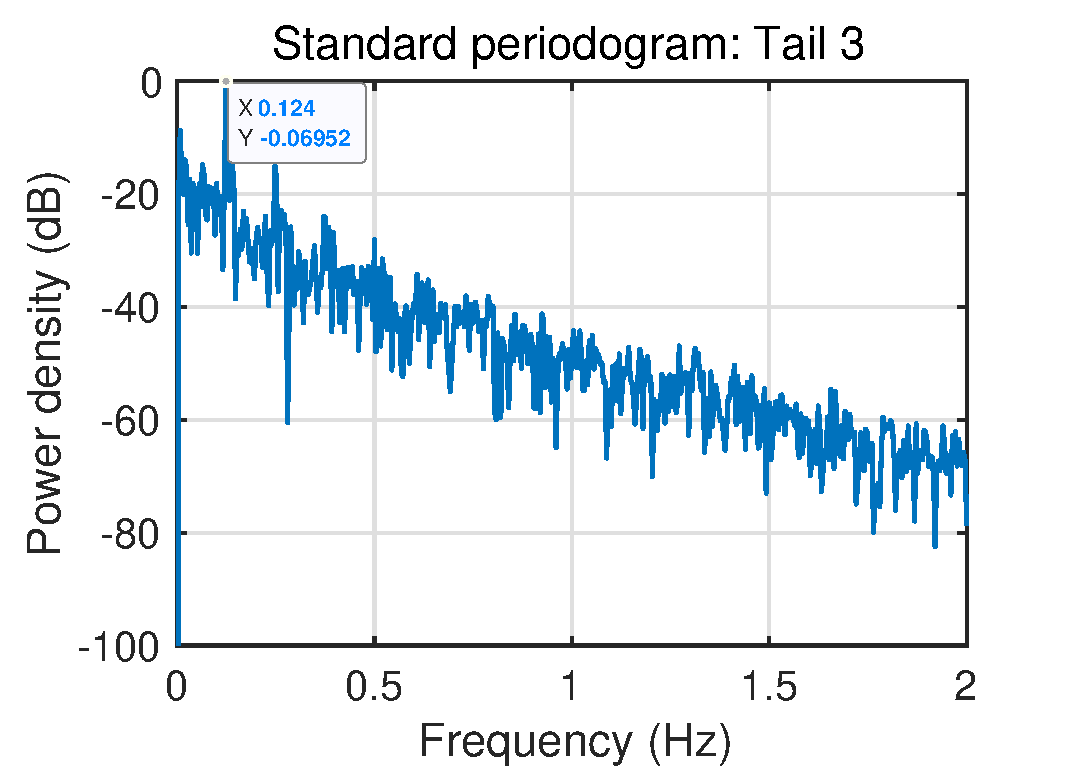
\includegraphics[width=\textwidth]{fig/15/15a5.eps}
     \end{subfigure}
     ~
     \begin{subfigure}{0.4\textwidth}
         \centering
         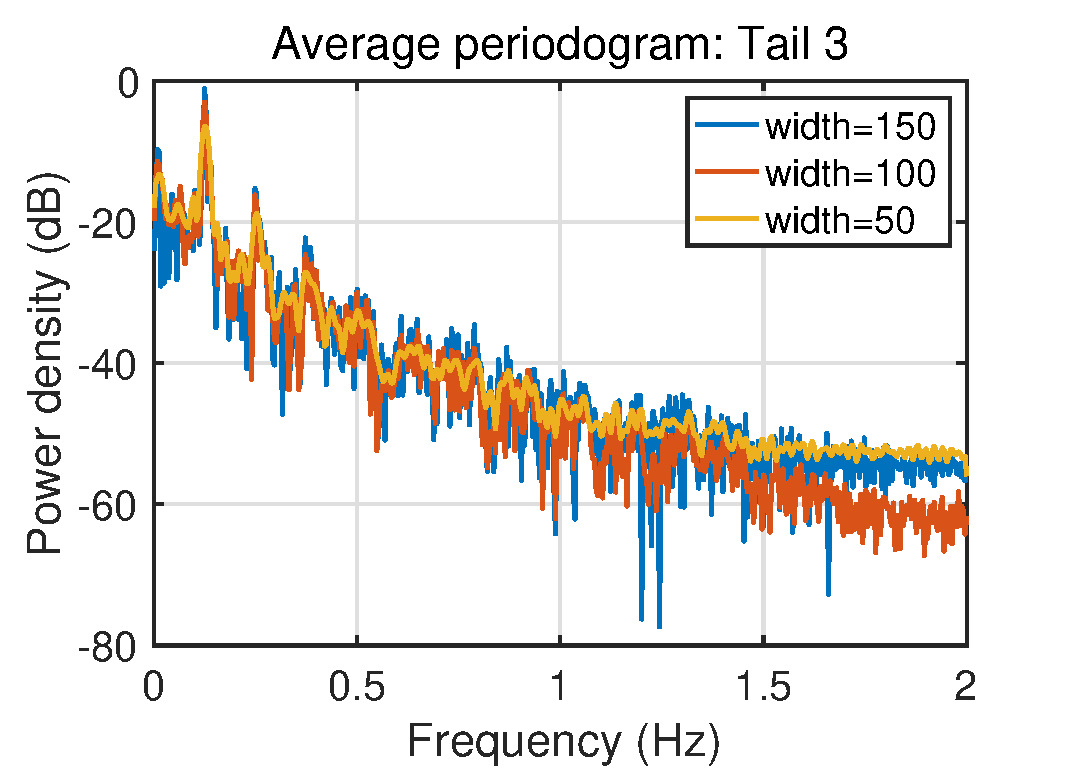
\includegraphics[width=\textwidth]{fig/15/15a6.eps}
     \end{subfigure}
        \caption{PSD of RRI data}
        \label{fig:1_5_a}
\end{figure}
\subsection{Frequency of three trails}
The experiment recorded the ECG data of three trails with normal, fast and slow breathing respectively. Therefore, the breaths per minute (BMP) for three trails will be different. A range of $12 \sim 20$ BMP is considered as the reference range for the normal breath. The observed peaks for three trails are $0.192Hz$, $0.416Hz$ and $0.124Hz$, corresponding to 23.04, 49.92 and 14.88 in BMP respectively. However, the harmonics frequencies of Trail 1 are failed to be captured which is probably caused by no restriction of the breath experiment. Trail 2 illustrate one harmonic at $f=0.832Hz$ and a large response at $0.928Hz$ at the same time, reasons of which may be the noise and the resolution of window. In addition, Trail 3 detects three harmonics frequencies at $0.248Hz$, $0.372Hz$ and $0.496Hz$.
\subsection{AR modelling of RRI data}
Fig.\ref{fig:1_5_c} depicts the AR model estimations with the incremental of order $p$. For Trail 1, the optimal order $p=10$ which detects the approximate peak at $f=0.192Hz$. The order of Trail 2 at $p=6$ can only detect the fundamental peak while harmonics can be detected with higher order. As to Trail 3, only when the order $p\ge2$, the peaks can be identified whereas the harmonics are difficult to be detected even if the order is high. Hence, the under-modelling causes the failed detection of peak and the over-modelling leads to capture harmonics and noise peaks. Compared with standard and averaging periodogram methods, the AR model performs powerfully in detecting interest peak and reducing variance as long as the order is determined.
\begin{figure}[t]
     \centering
     \begin{subfigure}[b]{0.4\textwidth}
         \centering
         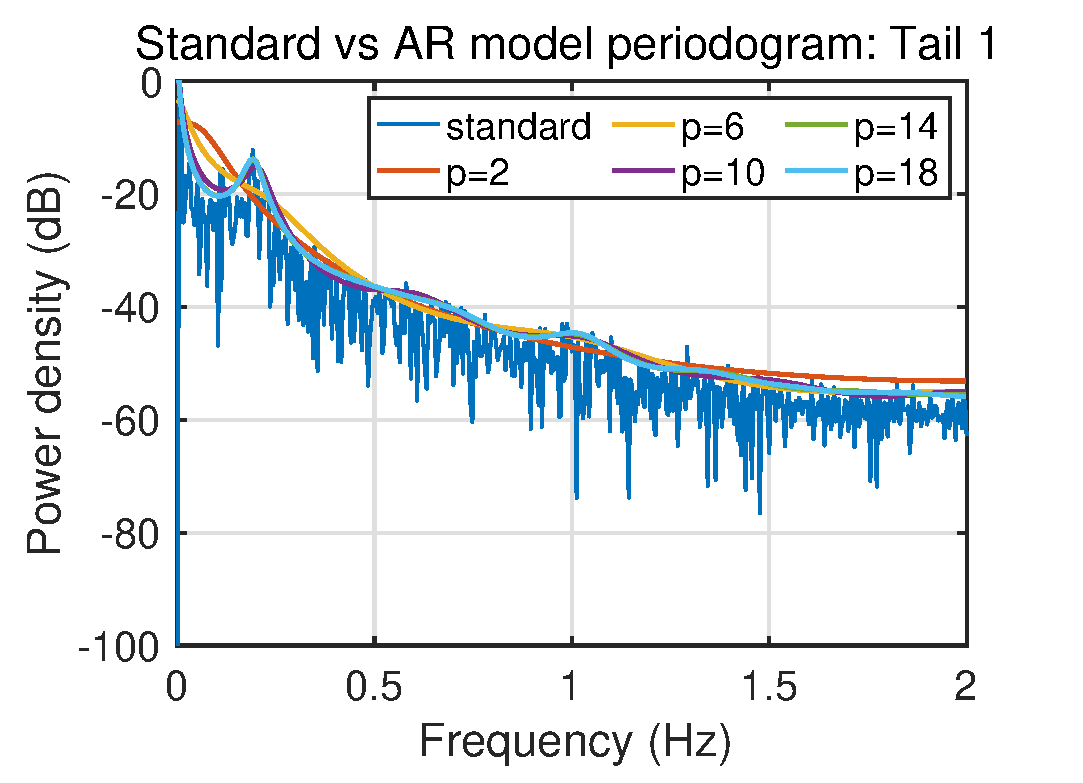
\includegraphics[width=\textwidth]{fig/15/15c1.eps}
     \end{subfigure}
     ~
     \begin{subfigure}[b]{0.4\textwidth}
         \centering
         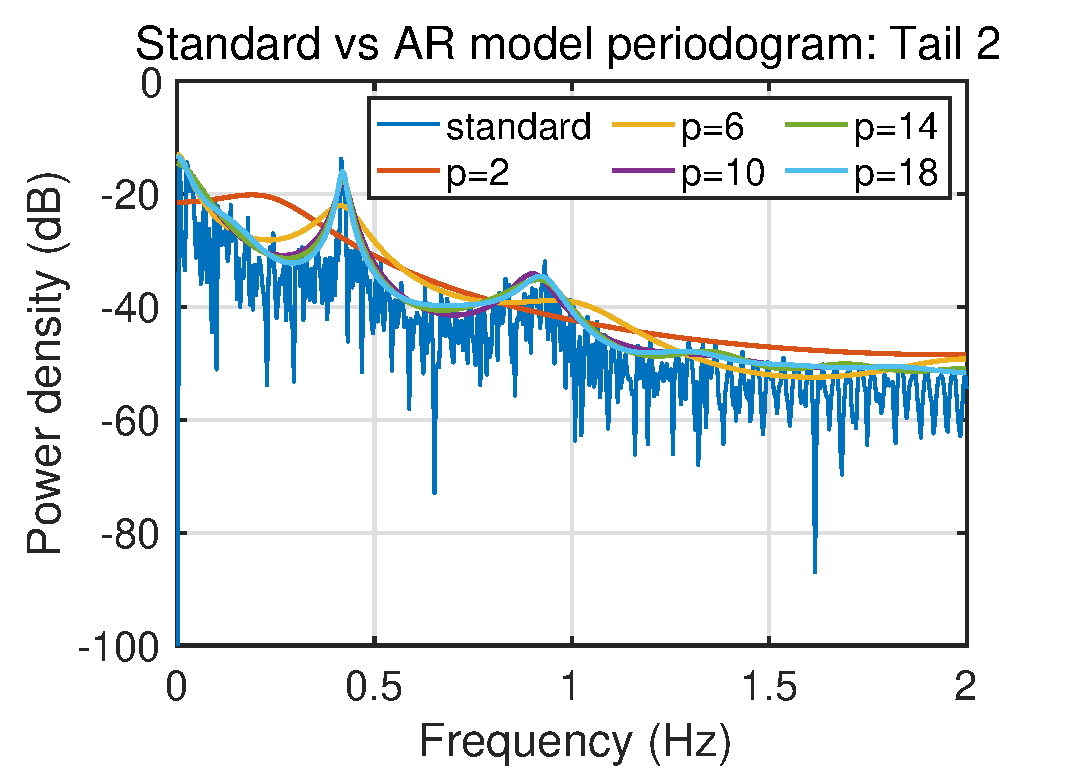
\includegraphics[width=\textwidth]{fig/15/15c2.eps}
     \end{subfigure}
     ~
     \begin{subfigure}[b]{0.4\textwidth}
         \centering
         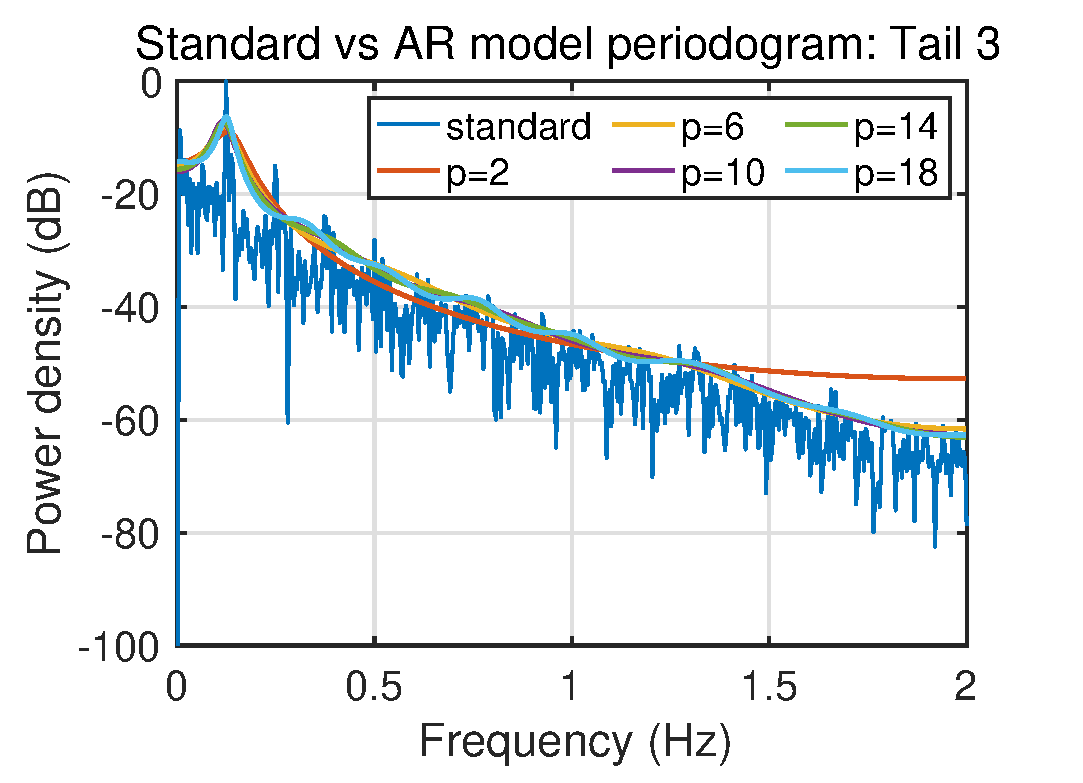
\includegraphics[width=\textwidth]{fig/15/15c3.eps}
     \end{subfigure}
        \caption{AR Model of RRI data}
        \label{fig:1_5_c}
\end{figure}










